\documentclass[a4paper,12pt]{article}
\usepackage[francais]{babel} % Package babel pour le français
\usepackage[T1]{fontenc}    % Package pour les accentuations
\usepackage[utf8]{inputenc}  % Français
\usepackage{textcomp}
\usepackage{lmodern}        % Pour avoir de bonnes polices en pdf
\usepackage{graphicx}       % Indispensable pour les figures
\usepackage{epstopdf}       % Utile pour les figures, résout une erreur
\usepackage{amsmath}        % Environnement pour les maths, permet du mettre du texte dans les équations
\usepackage{dialogue}		% Pour les dialogues
\usepackage{geometry}       % Utilisé pour les marges
\usepackage{pst-tree}		% Pour dessiner des arbres
\usepackage{pst-node}
\usepackage{multicol}		% Pour les colonnes
\usepackage{mathtools, bm}  % Typographie pour les ensembles communs
\usepackage{amssymb, bm}    % Typographie pour les ensembles communs
\usepackage{float}          % Pour bien placer les figures, scripts et tableaux
%\usepackage{listings}       % Utilisé pour les scripts
\usepackage{wrapfig}
\usepackage{xcolor}
\usepackage[french,onelanguage,ruled,vlined]{algorithm2e} %Pour les algorithmes
\definecolor{vertclair}{rgb}{0.10,0.55,0.17}
\definecolor{vertfonce}{rgb}{0,0.44,0}
\definecolor{grisclair}{rgb}{0.78,0.78,0.78}
\definecolor{prune}{rgb}{0.65,0.00,0.00}
\definecolor{bleufonce}{rgb}{0.06,0.06,1.00}
\definecolor{violet}{rgb}{0.21,0.18,0.73}
\definecolor{orange}{rgb}{0.93,0.46,0.00}

\usepackage{tikz}			%Pour les figures et graphes
\usetikzlibrary{calc}		%Pour les figures et graphes
\usepackage[cache=false]{minted}        % Utilisé pour les scripts
\geometry{hmargin=2cm,vmargin=2cm} % Réglages des marges
\usepackage{fancyhdr}		% Pour l'entête et les pieds de page
\pagestyle{fancy}			% Pour l'entête et les pieds de page
\usepackage{hyperref}		% Pour les liens hypertext, sommaire et références
\usepackage[final]{pdfpages} % Pour inclure des .pdf

\renewcommand{\abstractname}{Avant-propos} %Modification du titre de l'abstract
\newcommand{\norme}[1]{\left\Vert #1\right\Vert} %Commande pour la norme euclidienne
\renewcommand{\listoflistingscaption}{Liste des programmes} %Pour changer le titre de la liste des codes
\renewcommand{\listingscaption}{Programme} %Pour changer la légende des codes

\SetKwRepeat{doWhile}{faire}{tant que} % Pour les do-while


\newminted{console}{mathescape,

               breaklines = true,
               numbersep=5pt,
               frame=lines,
               framesep=2mm}

\newminted{lisp}{mathescape,

               breaklines = true,
               numbersep=5pt,
               frame=lines,
               framesep=2mm}

\renewcommand{\headrulewidth}{0.5pt}
\fancyhead[L]{IA01}
\fancyhead[R]{TP03 : Réalisation d’un système expert d’ordre $0+$}


\begin{document}


\thispagestyle{empty}

{\large

\vspace*{1cm}

\begin{center}

	{\bf Rapport de IA01 : \\Intelligence artificielle -- Représentation des connaissances}
	\vspace*{1cm}
	{\bf \\UNIVERSITE DE TECHNOLOGIE DE COMPIEGNE}

	\vspace*{1cm}
	
\includegraphics[scale=0.6]{UTC_logo.png}
	\vspace*{1cm}

	Automne 2016

	\vspace*{1cm}

	\vspace*{1cm}
	{\Large {\bf Guillaume JOUNEL \& Julien JERPHANION}}

	\vspace*{2 cm}
\end{center}

\flushleft{Sujet du rapport:\ \\
{\Large {\bf TP03 : Réalisation d’un système expert d’ordre $0+$}}}

\vspace*{1 cm}
\flushleft{Département des étudiants :\ \\
{\Large {\bf  Génie Informatique}}}\\

\vspace*{1 cm}
\flushleft{Professeur :\ \\
{\Large {\bf Marie-Hélène ABEL}}}\\
}

\newpage
\tableofcontents
%\newpage
%\listoffigures
\newpage
\listoflistings
\newpage

\section{Introduction : Présentation du système expert}


\subsection{Problématique}

Tous les programmeurs sont un jour confrontés au problème suivant :

\begin{quotation}
\centering
« \textit{Quels de programmation et technologies sont les plus adaptés pour le projet que je souhaite développer dans mon cadre d'utilisation ?} »

\end{quotation}


    Pour pallier à ce problème, nous allons concevoir un système expert qui propose différentes possibilités les plus adaptées selon l'usage.

    Pour cela, nous prendrons en compte de multiples critères tels que le domaine d'application (calcul numérique, intelligence artificielle...), l'expérience de l'utilisateur ou encore les caractéristiques de sa machine (Linux, MacOS...).

\subsection{Sources de connaissances sur le sujet}

    Les sources d'expertise ne manquent pas : il existe de nombreux sites et ressources sur le Net qui donnent les avantages et inconvénients de tous les langages de programmation existants selon les cas d'utilisation. En voici quelques uns :
    \begin{itemize}
        \item Wikipédia : Liste des langages de programmations par type :\\ \href{https://en.wikipedia.org/wiki/List_of_programming_languages_by_type}{\texttt{https://en.wikipedia.org/wiki/List\_of\_programming\_languages\_by\_type}} ;
        \item Learneroo: The Different Programming Languages :\\ \href{https://www.learneroo.com/modules/12/nodes/94}{\texttt{https://www.learneroo.com/modules/12/nodes/94}} ;
        \item WhoIsHostingThis: What Code Should You Learn?\\ \href{http://www.whoishostingthis.com/blog/2014/09/04/learn-to-code/}{\texttt{http://www.whoishostingthis.com/blog/2014/09/04/learn-to-code/}}.
    \end{itemize}


\section{Architecture}

\subsection{Rappels sur l'architecture}
Rappelons rapidement l'architecture d'un système expert.
Un système expert est constitué de trois parties principales dissociées les unes des autres : une \textit{base de faits}, une \textit{base de règles}, et un \textit{moteur d'inférences}.\\

La base de faits est une base d'informations qui comprend les faits initiaux et déduits au cours du programme.\\

La base de règles contient les différentes règles (connaissances implicites de l'expert rendues explicites pour être représentées informatiquement) utilisées pour déduire d'autres faits.\\

Les inférences au cours du processus sont réalisées par le moteur d'inférences. C'est lui qui fait le lien entre les deux précédentes bases. Il exécute les règles contenues dans la base de règles au regard des faits présents dans la base de faits ; les règles étant déclenchables en fonction des faits avérés. À la fait de l'exécution d'une règle, le résultat retourné qui est aussi un fait est stocké dans la base de faits.\\

Il existe de type de fonctionnement pour les moteurs d'inférences : le \textit{chaînage avant} et le \textit{chaînage arrière}.

Le chaînage avant consiste à regarder les faits présents et à choisir une règle qui peut être exécutée : on cherche les résultats que l'on peut obtenir en se basant sur les résultats déjà obtenus.

Le chaînage arrière examine les règles à exécuter pour arriver à un certain fait : on cherche un moyen d'arriver à un certain résultat.

\subsection{Base de faits}

Puisqu'il s'agit de concevoir un système expert d'ordre $0+$, nous avons choisi d'implémenter nos faits selon la forme suivante :

\begin{quotation}
	\mintinline{lisp}{(objet EQ valeur)}
\end{quotation}

La base de faits est stockée dans une variable globale \mintinline{lisp}{*faits*} initialement vide : elle se remplira au cours de l'exécution du système.

\subsection{Base de règles}
Nous avons décidé d'implémenter notre base de règle de cette façon :

\begin{minted}{lisp}
	(((Premisse1 operateur valeur)...(PremisseN operateur valeur))
  	  ((Resultat1 operateur valeur)...(Resultat1M operateur valeur)))
\end{minted}
où $\mintinline{lisp}{operateur} \in \{\mintinline{lisp}{=},\mintinline{lisp}{<},\mintinline{lisp}{>},\mintinline{lisp}{EQ}\} $.
\begin{listing}[H]
	\centering
	\inputminted[breaklines=true,linenos,lastline=29]{lisp}{../regles.lisp}
\end{listing}

\begin{listing}[H]
	\centering
	\inputminted[breaklines=true,linenos,firstline=30]{lisp}{../regles.lisp}
	\caption{Base de règles \mintinline{lisp}{*regles*}}
\end{listing}

\subsection{Base de connaissances}
Pour donner les informations concernant les technologies choisies par \textit{Cactus} nous avons décider d'implémenter une base de connaissances. Celle-ci contient pour chaque technologie une brève description de celle-ci.

Les éléments des cette base sont représentés sous la forme de liste pointée ainsi :

\begin{quotation}
	\mintinline{lisp}{(technologie . "La description de la technologie")}
\end{quotation}

\begin{listing}[H]
	\centering
	\inputminted[breaklines=true,linenos,lastline=26]{lisp}{../technologies.lisp}
	\caption{Base de connaissances \mintinline{lisp}{*technologies*}}
\end{listing}

\begin{listing}[H]
	\centering
	\inputminted[breaklines=true,linenos,firstline=27]{lisp}{../technologies.lisp}
	\caption{Base de connaissances \mintinline{lisp}{*technologies*}}
\end{listing}

Nous utiliserons cette base de connaissances dans la fonction \mintinline{lisp}{afficherPropositions} que nous détaillerons plus bas : l'idée est d'avoir un petit descriptif des technologies proposées pour comprendre en quoi elles sont pertinentes.


\section{Fonctionnement du système}

\subsection{Chaînage avant}

Voici un algorithme itératif pour le chaînage avant.
\begin{algorithm}
%\KwData{$[y_k]_{k\in I_n}$, le signal échantilloné (avec $I_n := \{1, \cdots, n\}$)}
%\KwResult{$[z_k]_{k\in I_n}$, }
\Begin{
	\doWhile{{\bf il n'y a pas de propositions dans $BF$\ }}{
		\For{{\bf chaque règle} $r$ {\bf de la base de règle $BR$}}{
			\If{r {\bf est déclenchable}}{
				$EC \leftarrow EC\ \cup \{r\}$\;
				$BR \leftarrow BR -\{r\}$\;
			}
			\eIf{$EC \neq \emptyset$}{
				$BF \leftarrow BF\ \cup$ {\bf conclusions(}$r${\bf )}\;
			}{
			{\bf poser une question}}\;
		}
	}

{\bf afficher les propositions} \;
}
\caption{Chaînage Avant \label{algoChainageAvant}}
\end{algorithm}

On remarquera que le système s'arrêtera dès que des propositions auront été inférées par le moteur.


Nous l'avons implémenté sous LISP de cette façon :

\begin{listing}[H]
	\centering
	\inputminted[breaklines=true,linenos]{lisp}{../chainageAvantLarg.lisp}
	\caption{Moteur de chainage avant}
\end{listing}

\subsection{Fonctions outils}

Afin d'abstraire les raisonnements nous avons mis au points des fonctions outils. \mintinline{lisp}{conclusion()}, \mintinline{lisp}{declenchable?()} et \mintinline{lisp}{ajouter()} sont celles mises en place pour les règles.
\begin{listing}[H]
	\centering
	\inputminted[breaklines=true,linenos]{lisp}{../fonctionsOutilsRegles.lisp}
	\caption{Fonctions outils pour les règles}
\end{listing}

\mintinline{lisp}{objet()}, \mintinline{lisp}{operateur()} et \mintinline{lisp}{valeur()} sont celles mises en place pour les faits.

\begin{listing}[H]
	\centering
	\inputminted[breaklines=true,linenos]{lisp}{../fonctionsOutilsFaits.lisp}
	\caption{Fonctions outils pour les faits}
\end{listing}

\subsection{Poser une question : fonction \mintinline{lisp}{askQuestion}}

Une possibilité lorsque le système n'arrive plus à tirer de conclusions et de poser des questions à l'utilisateur pour apporter de nouveaux faits. C'est ici le rôle réalisé par la fonction \mintinline{lisp}{askQuestion}.

\begin{listing}[H]
	\centering
	\inputminted[breaklines=true,linenos, firstline = 22]{lisp}{../askQuestion.lisp}
	\caption{Fonction \mintinline{lisp}{askQuestion} permettant de récupérer des informations}
\end{listing}

Nous utilisons d'autres fonctions pour réaliser certaines tâches.

\begin{listing}[H]
	\centering
	\inputminted[breaklines=true,linenos, lastline = 21]{lisp}{../askQuestion.lisp}
	\caption{Fonctions outils pour \mintinline{lisp}{askQuestion}}
\end{listing}

\subsection{Afficher les propositions du système : fonction \mintinline{lisp}{afficherPropositions}}

	C'est dans cette fonction que nous utilisons la base de connaissances \mintinline{lisp}{**technologies**}.

\begin{listing}[H]
	\centering
	\inputminted[breaklines=true,linenos]{lisp}{../afficherPropositions.lisp}
	\caption{Fonction \mintinline{lisp}{afficherPropositions} qui affiche les propositions du système expert}
\end{listing}


\[ \star \quad \star \quad \star \]
\newpage
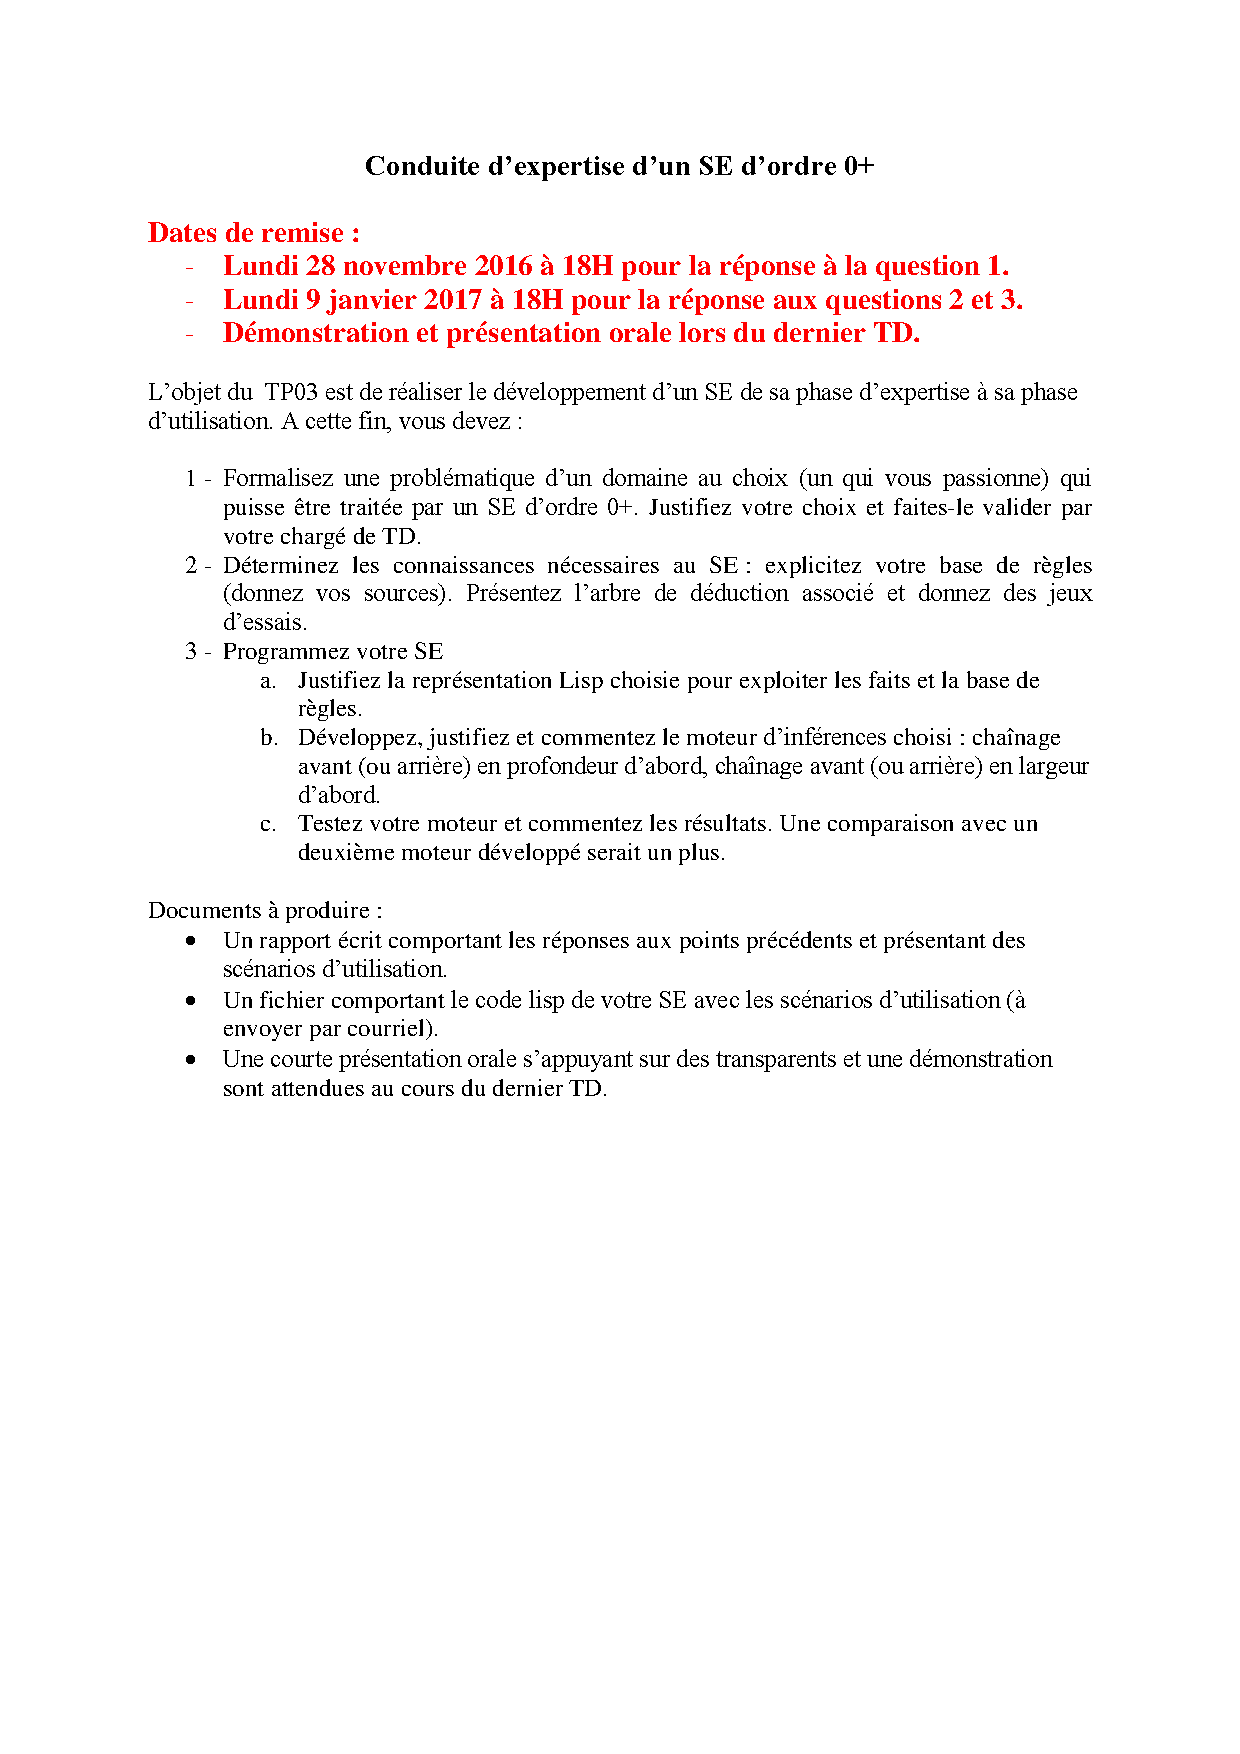
\includepdf[pages=1]{sujet.pdf}
\end{document}
